\begin{frame}[fragile]{Tutorial: Two-site operators}

\begin{columns}

\begin{column}{5cm}

\begin{onlyenv}<1-2>
\begin{lstlisting}[language=JuliaLocal, style=julia, basicstyle=\scriptsize\ttfamily]
inner(Zp1' * Zp2', H,
      Zp1 * Zp2)
\end{lstlisting}
\end{onlyenv}

\begin{onlyenv}<3->
\begin{lstlisting}[language=JuliaLocal, style=julia, mathescape, basicstyle=\scriptsize\ttfamily]
D, _ = eigen(H);
diag(D) $\approx$ [-√2, -1, 1, √2]
\end{lstlisting}
\end{onlyenv}

\end{column}

\begin{column}{5cm}

\begin{onlyenv}<1-1>
$\langle$Z+Z+|H|Z+Z+$\rangle$ \\
\end{onlyenv}

\begin{onlyenv}<2-2>
\vspace*{0.0cm}
\begin{center}
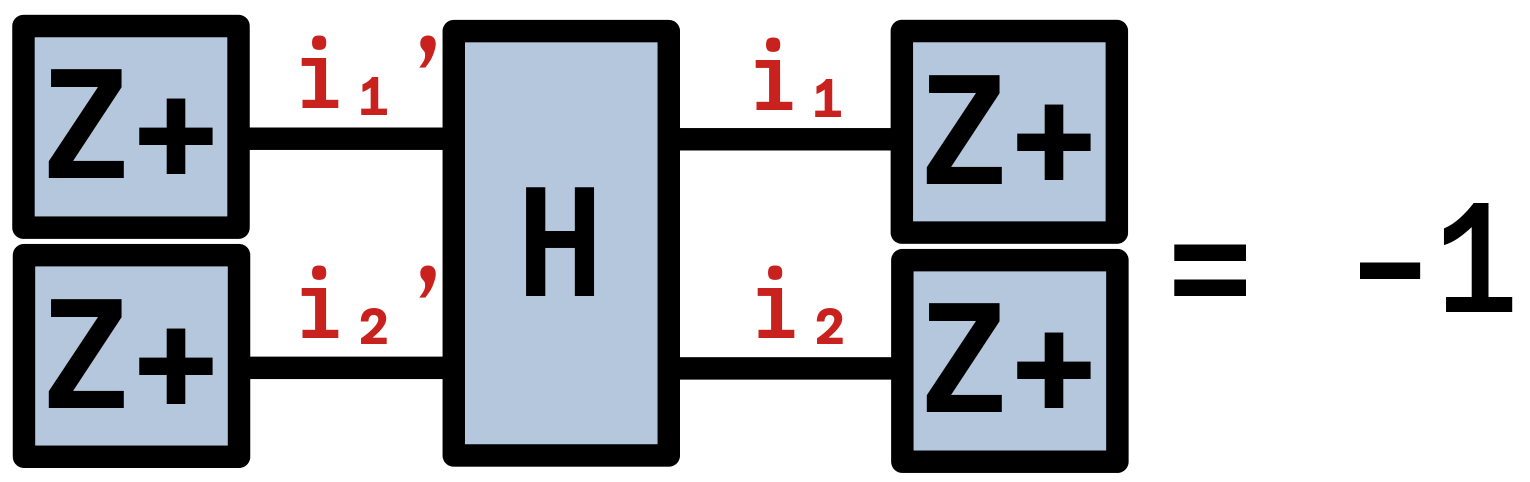
\includegraphics[width=1.0\textwidth]{
  slides/assets/Zp1Zp2HZp1Zp2.png
}
\end{center}
\vspace*{0.0cm}
\end{onlyenv}

%% \begin{onlyenv}<3-3>
%% ~\\
%% $\approx$ [-√2, -1, 1, √2]
%% \end{onlyenv}

\begin{onlyenv}<3->
\vspace*{0.0cm}
\begin{center}
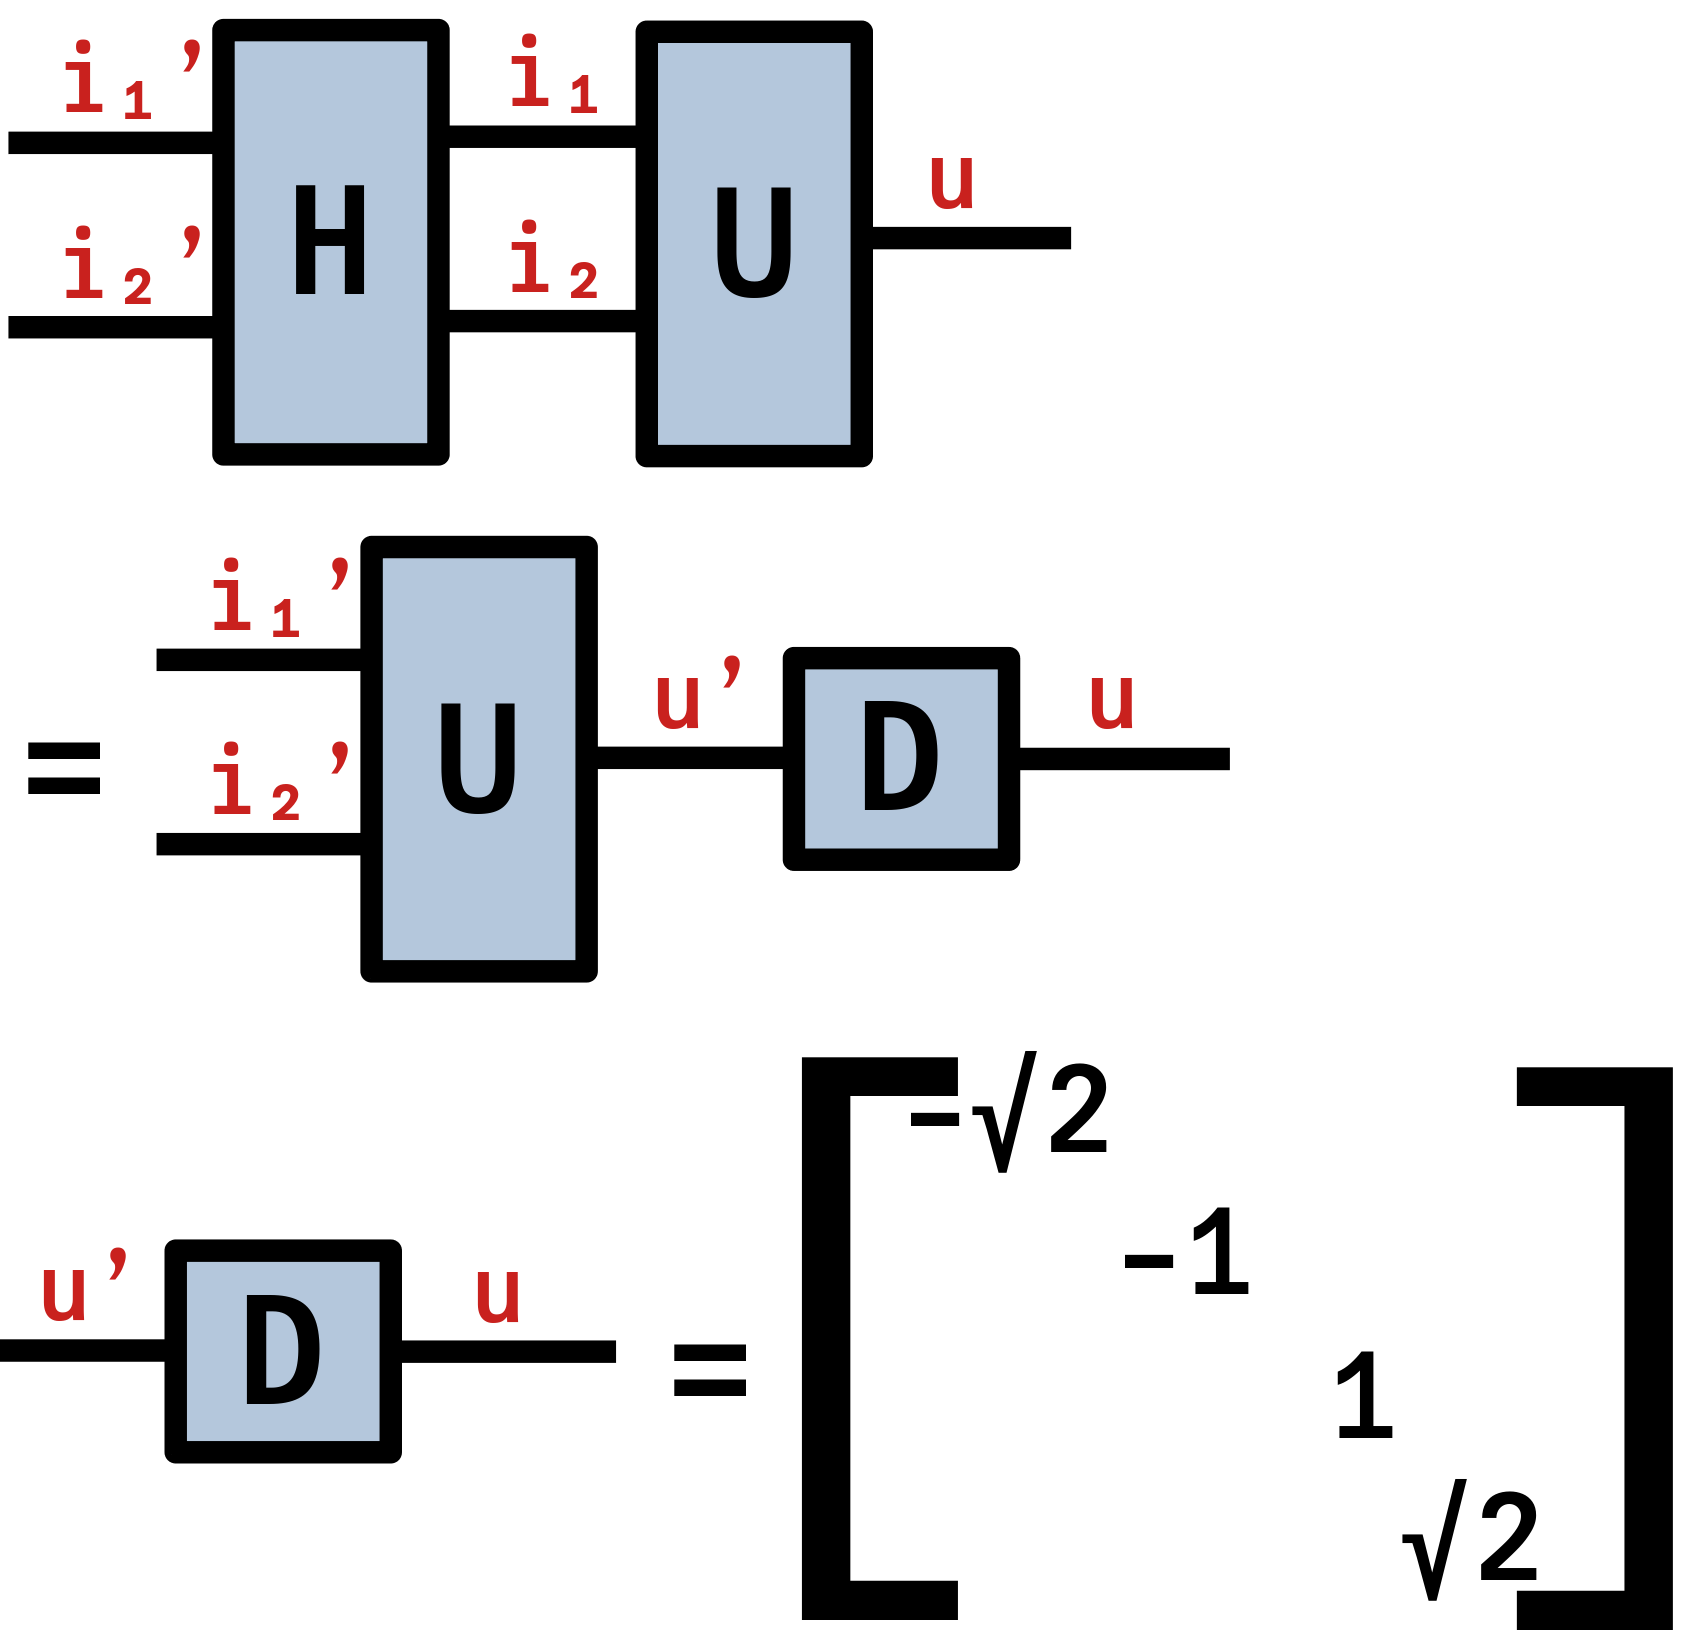
\includegraphics[width=1.0\textwidth]{
  slides/assets/eigen_H.png
}
\end{center}
\vspace*{0.0cm}
\end{onlyenv}

\end{column}

\end{columns}

\end{frame}
